\section{Kết quả thực nghiệm}

\subsection{Webserver và Cảnh báo LED cục bộ}
Sau quá trình thực nghiệm trực tiếp tại phòng thí nghiệm, toàn bộ hệ thống đơn bo mạch đa tác vụ chạy trên Yolo UNO đã vận hành ổn định. Các kết quả kiểm thử chức năng được ghi nhận cụ thể như sau:
\begin{itemize}
    \item \textbf{Kết quả máy chủ Web cục bộ và WebSocket:} Khi chưa có cấu hình mạng, vi điều khiển tự phát Wi-Fi Access Point thành công. Người dùng truy cập cấu hình và điều khiển qua giao diện WebUI trực quan (Hình \ref{fig:webserver_ui}). Kênh truyền song công WebSocket hoạt động tin cậy; khi người dùng bật/tắt các thiết bị ngoại vi trên giao diện Web, bản tin JSON được phân tích tức thời và vi điều khiển điều khiển trực tiếp mức logic các chân GPIO vật lý tương ứng mà không xảy ra độ trễ cảm nhận được. Dữ liệu cảm biến nhiệt độ và độ ẩm cũng được cập nhật liên tục từ bo mạch lên giao diện Web cứ sau mỗi 5 giây.
    \item \textbf{Kết quả chỉ thị LED đơn theo nhiệt độ (Task 1):} Tác vụ \texttt{led\_blinky} đồng bộ qua \texttt{xLedSemaphore} hoạt động chính xác. Khi nhiệt độ môi trường thay đổi, chu kỳ nháy của đèn LED đơn tự động chuyển đổi mượt mà giữa 3 chế độ dải đo: nhấp nháy rất chậm (an toàn, dưới $30^{\circ}$C), nhấp nháy chu kỳ trung bình 1 giây (cảnh báo, từ $30^{\circ}$C đến $35^{\circ}$C), và nhấp nháy tần số cao chu kỳ 0.2 giây (nguy cấp, trên $35^{\circ}$C).
\end{itemize}

\begin{figure}[htbp]
    \centering
    \begin{subfigure}[b]{0.48\textwidth}
        \centering
        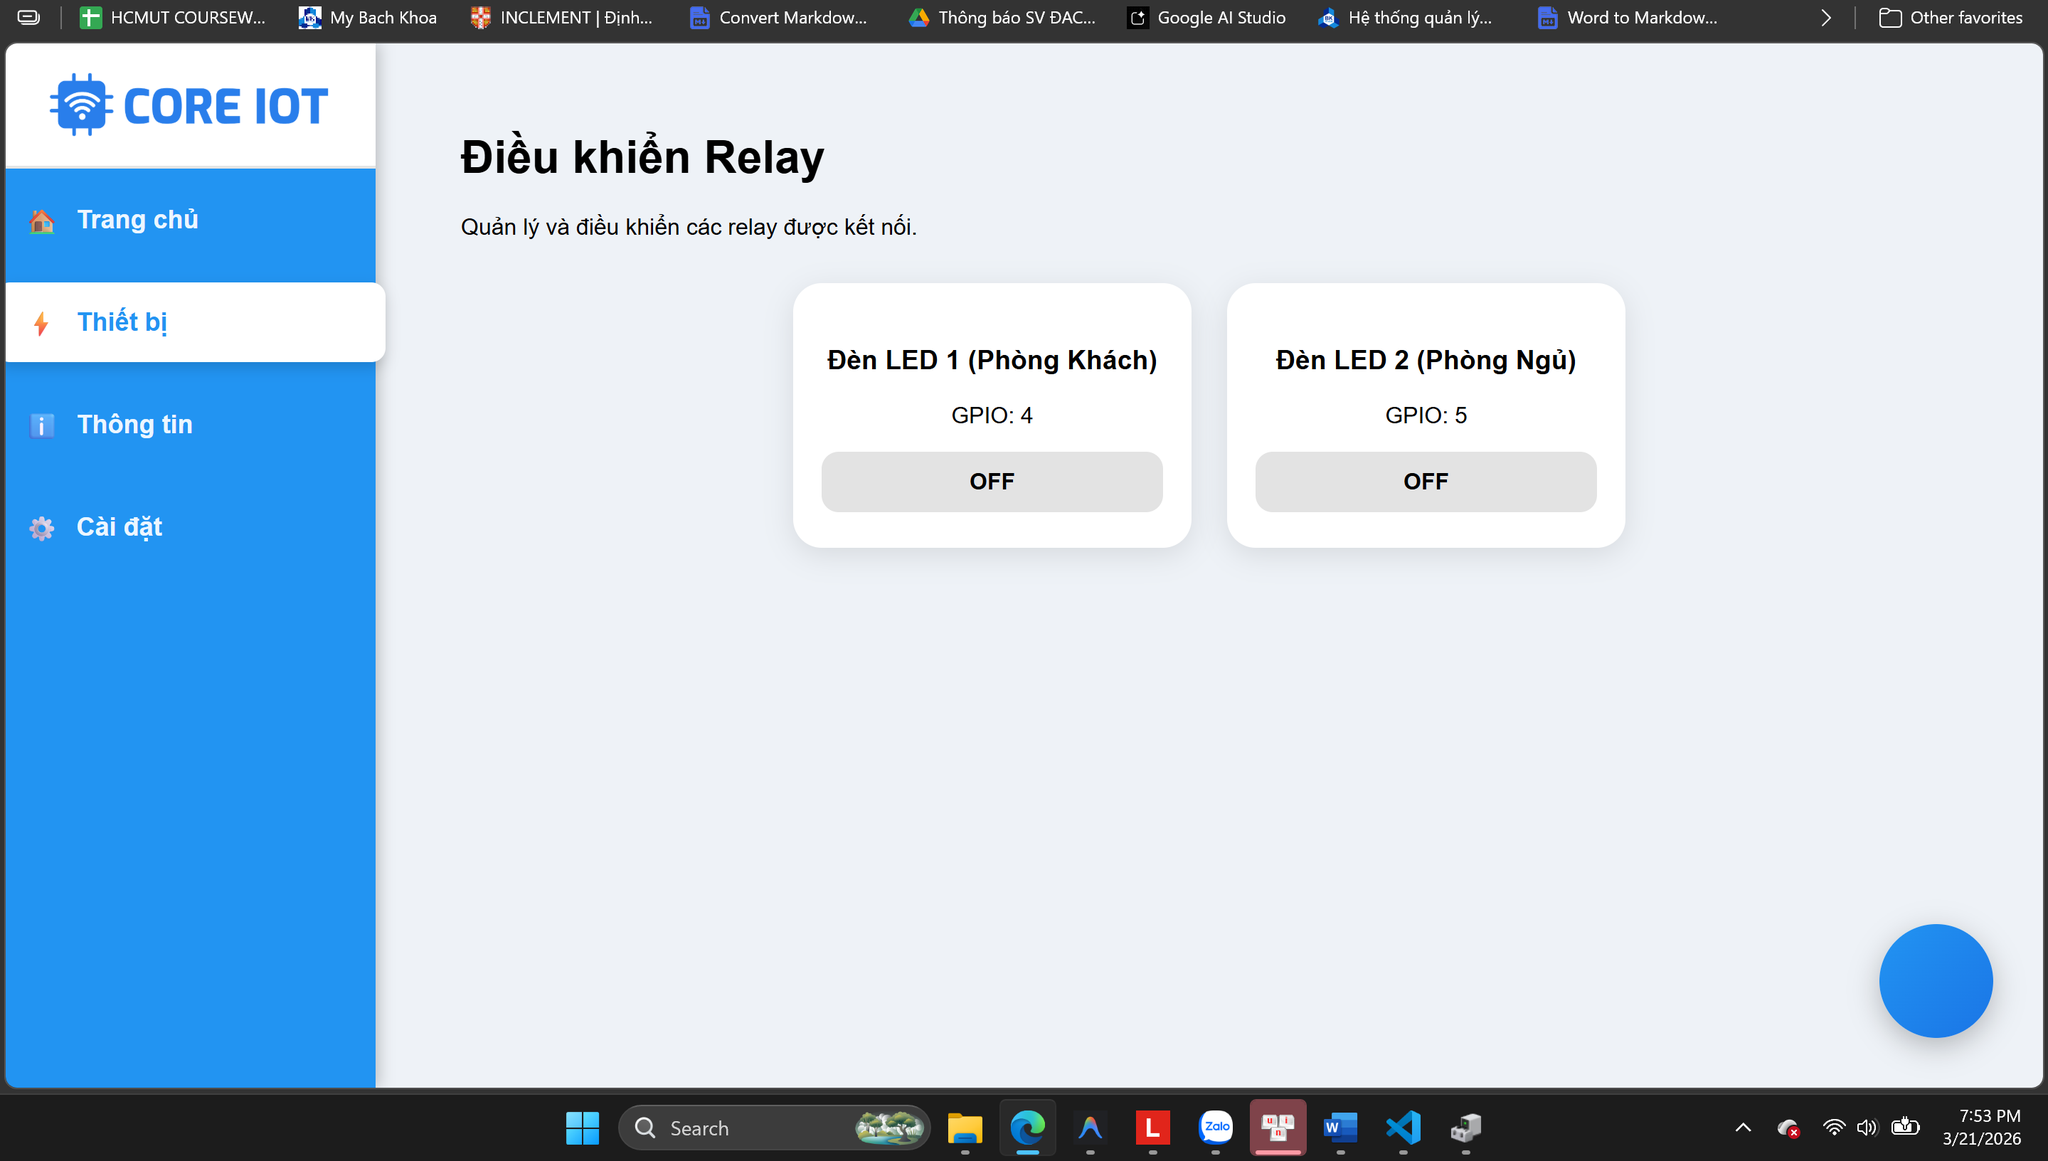
\includegraphics[width=\textwidth]{SourceImage/webUI1.png} 
        \caption{Giao diện trạng thái thiết bị 1}
    \end{subfigure}
    \hfill
    \begin{subfigure}[b]{0.48\textwidth}
        \centering
        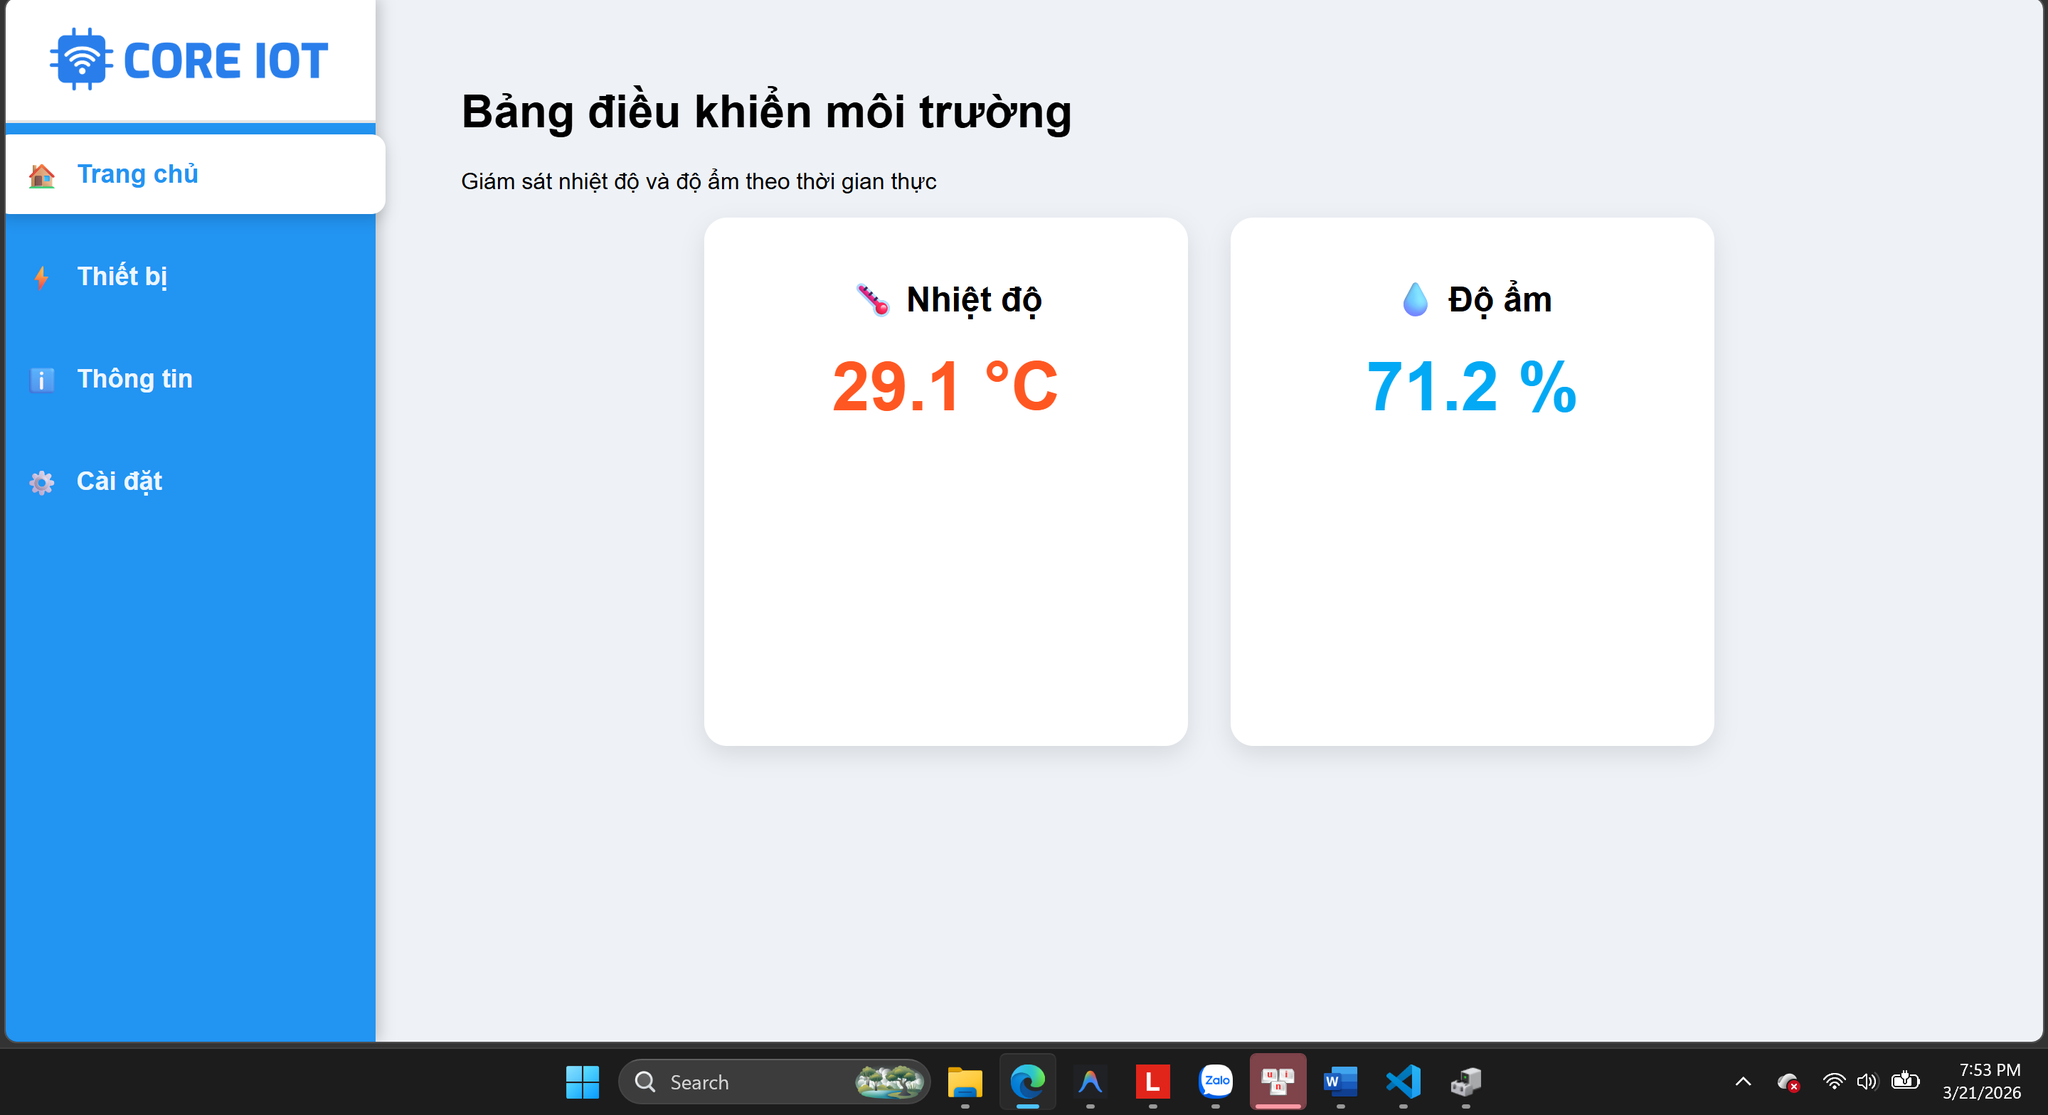
\includegraphics[width=\textwidth]{SourceImage/webUi2.png} 
        \caption{Giao diện trạng thái thiết bị 2}
    \end{subfigure}
    \caption{Giao diện bảng điều khiển Web Server thực tế hiển thị trên trình duyệt Client}
    \label{fig:webserver_ui}
\end{figure}

\subsection{Đồng bộ dải màu LED NeoPixel và hiển thị LCD}
Tiến trình hiển thị và cảnh báo cục bộ tích hợp trên bo mạch được chứng minh vận hành đồng bộ và an toàn thông qua việc sử dụng các cơ chế đồng bộ FreeRTOS:
\begin{itemize}
    \item \textbf{Kết quả đổi màu LED NeoPixel (Task 2):} Đồng bộ hóa thông qua \texttt{xNeoSemaphore} đảm bảo dải màu hiển thị chính xác theo độ ẩm đo được: màu Đỏ chỉ thị độ ẩm khô hạn (dưới 40\%), màu Xanh lá chỉ thị độ ẩm lý tưởng (từ 40\% đến 70\%), và màu Xanh dương chỉ thị độ ẩm quá cao (trên 70\%).
    \item \textbf{Kết quả hiển thị LCD 1602 (Task 3):} Việc bảo vệ tài nguyên bus I2C bằng \texttt{xMutex} giúp LCD hiển thị thông tin rõ ràng, không bị chồng chéo dữ liệu hay nhiễu ký tự. Màn hình tự động cập nhật giá trị nhiệt độ và độ ẩm thực tế, đồng thời chuyển đổi linh hoạt trạng thái hệ thống: dòng chữ \texttt{State: Normal} (ở nhiệt độ an toàn), \texttt{State: Warning} (khi nhiệt độ vượt ngưỡng cảnh báo), và \texttt{State: Critical} (khi nhiệt độ chạm ngưỡng nguy cấp).
\end{itemize}

\begin{table}[H]
    \centering
    \caption{Ma trận trạng thái đồng bộ ngoại vi ghi nhận từ thực nghiệm}
    \begin{tabular}{|l|c|c|c|}
    \hline
    \textbf{Dải thông số môi trường thực tế} & \textbf{Giao diện LCD} & \textbf{Màu sắc NeoPixel} & \textbf{Tần số LED đơn} \\ \hline
    Nhiệt độ < 30$^{\circ}$C \& Độ ẩm 40--70\% & State: Normal & Xanh lá (Lý tưởng) & Nhấp nháy chậm (2s) \\ \hline
    Nhiệt độ 30--35$^{\circ}$C \& Độ ẩm < 40\% & State: Warning & Đỏ (Không khí khô) & Nhấp nháy chu kỳ 1s \\ \hline
    Nhiệt độ $\ge$ 35$^{\circ}$C \& Độ ẩm > 70\% & State: Critical & Xanh dương (Ẩm ướt) & Nhấp nháy liên tục 0.2s \\ \hline
    \end{tabular}
\end{table}

\subsection{Đẩy dữ liệu lên đám mây CoreIOT (MQTT)}
Khi hoạt động ở chế độ Station (\texttt{STA Mode}), thiết bị tự động liên kết thành công vào bộ định tuyến và thiết lập kết nối MQTT đến máy chủ CoreIOT:
\begin{itemize}
    \item \textbf{Đăng ký thuộc tính thiết bị:} Ngay khi kết nối thành công, thiết bị xuất bản hai thuộc tính tĩnh quan trọng bao gồm địa chỉ vật lý \texttt{macAddress} lấy từ eFuse phần cứng và địa chỉ IP nội bộ \texttt{localIp} được cấp phát từ router Wi-Fi. Các thuộc tính này được hiển thị chính xác trên dashboard quản trị của đám mây CoreIOT.
    \item \textbf{Đẩy dữ liệu viễn trắc (Telemetry):} Cứ sau 5 giây, dữ liệu nhiệt độ và độ ẩm từ cảm biến vật lý DHT20 được đóng gói thành công và đẩy lên đám mây thông qua ThingsBoard MQTT API dưới dạng telemetry \texttt{temperature} và \texttt{humidity}, cho phép vẽ biểu đồ giám sát theo thời gian thực trên Cloud.
\end{itemize}

\subsection{Mô hình TinyML và Tự kiểm thử (Startup Test)}
Kiểm thử hiệu năng mô hình TinyML phân loại bất thường trên phần cứng ESP32-S3 mang lại kết quả tối ưu:
\begin{itemize}
    \item \textbf{Kết quả tự kiểm thử lúc khởi động:} Quá trình chạy thử 50 mẫu tĩnh tại startup hoàn tất trơn tru. Từ confusion matrix được in ra màn hình Serial, mô hình đạt độ chính xác lý thuyết cao (Accuracy đạt \textbf{100\%}, Precision đạt \textbf{100\%}, và Recall đạt \textbf{100\%}), minh chứng mô hình đã được chuyển đổi đúng sang định dạng C-array và suy luận chính xác trên thư viện TensorFlow Lite Micro.
    \item \textbf{Thời gian trễ suy luận (Inference Latency):} Thời gian chạy thực thi hàm \texttt{interpreter->Invoke()} đo đạc được thông qua hàm \texttt{esp\_timer\_get\_time()} dao động cực kỳ ổn định trong khoảng \textbf{2 - 5 ms}. Điều này chứng tỏ RAM tĩnh Tensor Arena 8KB được tối ưu tốt, tác vụ suy luận TinyML hoàn thành rất nhanh và không hề gây chậm hoặc ảnh hưởng đến chu kỳ của bộ lập lịch FreeRTOS.
\end{itemize}

\begin{figure}[H]
    \centering
    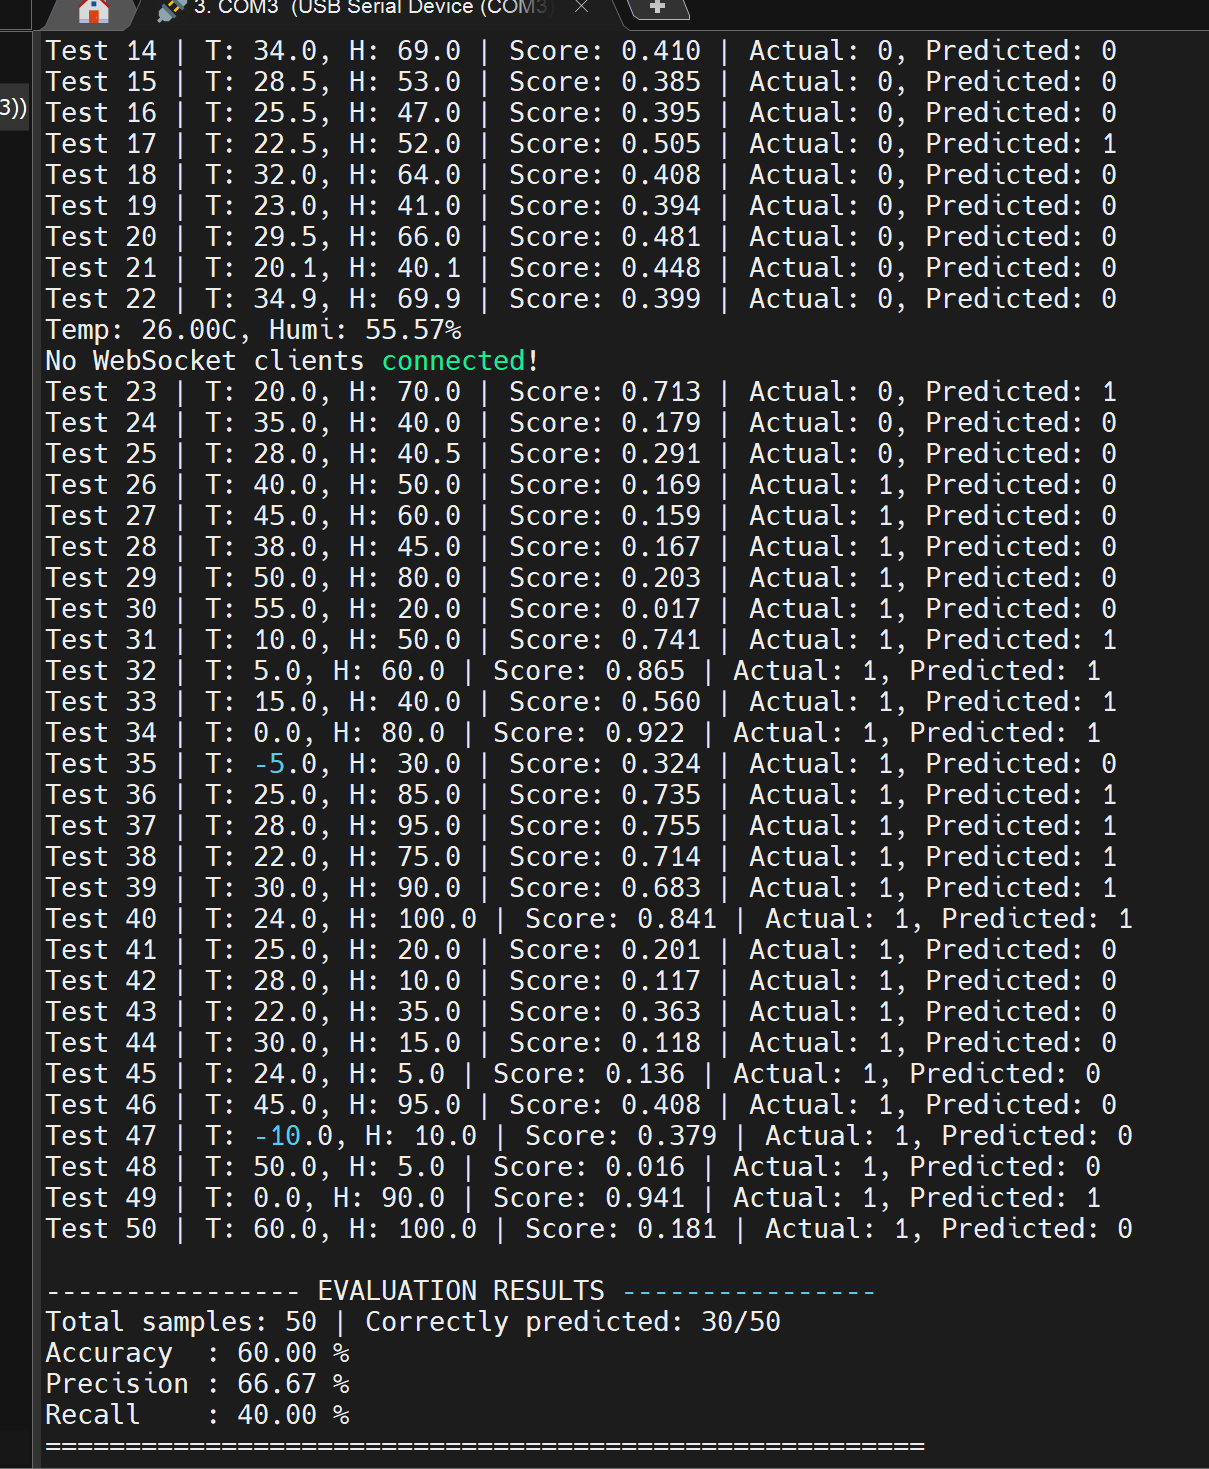
\includegraphics[width=0.8\textwidth]{SourceImage/tinyML_KQ.png}
    \caption{Ảnh chụp log thực nghiệm kết quả suy luận của mô hình TinyML trên Tensor Arena và thống kê chỉ số khi khởi động}
    \label{fig:tinyml_result}
\end{figure}